%%
%% This is file `sample-sigconf.tex',
%% generated with the docstrip utility.
%%
%% The original source files were:
%%
%% samples.dtx  (with options: `sigconf')
%%
%% IMPORTANT NOTICE:
%%
%% For the copyright see the source file.
%%
%% Any modified versions of this file must be renamed
%% with new filenames distinct from sample-sigconf.tex.
%%
%% For distribution of the original source see the terms
%% for copying and modification in the file samples.dtx.
%%
%% This generated file may be distributed as long as the
%% original source files, as listed above, are part of the
%% same distribution. (The sources need not necessarily be
%% in the same archive or directory.)
%%
%% The first command in your LaTeX source must be the \documentclass command.
\documentclass[sigconf,10pt]{acmart}

\settopmatter{printfolios=true}

\usepackage{hyperref}


\providecommand{\tightlist}{%
  \setlength{\itemsep}{0pt}\setlength{\parskip}{0pt}}

%%
%% \BibTeX command to typeset BibTeX logo in the docs
\AtBeginDocument{%
  \providecommand\BibTeX{{%
    \normalfont B\kern-0.5em{\scshape i\kern-0.25em b}\kern-0.8em\TeX}}}

%% Rights management information.  This information is sent to you
%% when you complete the rights form.  These commands have SAMPLE
%% values in them; it is your responsibility as an author to replace
%% the commands and values with those provided to you when you
%% complete the rights form.


%%
%% Submission ID.
%% Use this when submitting an article to a sponsored event. You'll
%% receive a unique submission ID from the organizers
%% of the event, and this ID should be used as the parameter to this command.
%%\acmSubmissionID{123-A56-BU3}

%%
%% The majority of ACM publications use numbered citations and
%% references.  The command \citestyle{authoryear} switches to the
%% "author year" style.
%%
%% If you are preparing content for an event
%% sponsored by ACM SIGGRAPH, you must use the "author year" style of
%% citations and references.
%% Uncommenting
%% the next command will enable that style.
%%\citestyle{acmauthoryear}
\pagenumbering{gobble}
%%
%% end of the preamble, start of the body of the document source.
\begin{document}

%%
%% The "title" command has an optional parameter,
%% allowing the author to define a "short title" to be used in page headers.
\title{Joker: A Unified Interaction Model For Web Customization}

%%
%% The "author" command and its associated commands are used to define
%% the authors and their affiliations.
%% Of note is the shared affiliation of the first two authors, and the
%% "authornote" and "authornotemark" commands
%% used to denote shared contribution to the research.

%\author{Kapaya Katongo}
%\affiliation{%
%  \institution{MIT CSAIL}
%  \city{Cambridge, MA}
%  \country{USA}
%}
%\email{kkatongo@mit.edu}

%\author{Geoffrey Litt}
%\affiliation{%
%  \institution{MIT CSAIL}
%  \city{Cambridge, MA}
%  \country{USA}
%}
%\email{glitt@mit.edu}

%\author{Kathryn Jin}
%\affiliation{%
%  \institution{MIT CSAIL}
%  \city{Cambridge, MA}
%  \country{USA}
%}
%\email{kjin@mit.edu}

%\author{Daniel Jackson}
%\affiliation{%
% \institution{MIT CSAIL}
%  \city{Cambridge, MA}
%  \country{USA}
%}
%\email{dnj@csail.mit.edu}

%%
%% By default, the full list of authors will be used in the page
%% headers. Often, this list is too long, and will overlap
%% other information printed in the page headers. This command allows
%% the author to define a more concise list
%% of authors' names for this purpose.
% \renewcommand{\shortauthors}{Trovato and Tobin, et al.}

%%
%% The abstract is a short summary of the work to be presented in the
%% article.
%% \begin{abstract}
%%  
%% \end{abstract}

%%
%% The code below is generated by the tool at http://dl.acm.org/ccs.cfm.
%% Please copy and paste the code instead of the example below.
%%
%% From HERE
%%\begin{CCSXML}
%%<ccs2012>
%%<concept>
%%<concept_id>10011007.10011006.10011066.10011069</concept_id>
%%<concept_desc>Software and its engineering~Integrated and visual development environments</concept_desc>
%%<concept_significance>500</concept_significance>
%%</concept>
%%</ccs2012>
%%\end{CCSXML}

%% \ccsdesc[500]{Software and its engineering~Integrated and visual development environments}
% To HERE

%%
%% Keywords. The author(s) should pick words that accurately describe
%% the work being presented. Separate the keywords with commas.
%% \keywords{end-user programming, software customization, web scraping, programming-by-example, program synthesis}

%% A "teaser" image appears between the author and affiliation
%% information and the body of the document, and typically spans the
%% page.
% \begin{teaserfigure}
%  \includegraphics[width=\textwidth]{sampleteaser}
%  \caption{Seattle Mariners at Spring Training, 2010.}
%  \Description{Enjoying the baseball game from the third-base
%  seats. Ichiro Suzuki preparing to bat.}
%  \label{fig:teaser}
%\end{teaserfigure}

%%
%% This command processes the author and affiliation and title
%% information and builds the first part of the formatted document.
\maketitle

\hypertarget{sec:introduction}{%
\section{Introduction}\label{sec:introduction}}

Many websites do not meet the exact needs of all of their users, so
millions of people use browser extensions and userscripts
\citep{zotero-224, 2021f} to customize them. However, these tools only
allow end-users to install customizations built by programmers. End-user
web customization systems like Sifter \citep{huynh2006}, Vegemite
\citep{lin2009} and Wildcard \citep{litt2020} provide a more accessible
approach, allowing anyone to create bespoke customizations without
performing traditional programming.

These tools each provide different useful mechanisms for end-user
customization, but they share a common design limitation: they have a
rigid separation between the two stages of the web customization
process. First, in the \emph{extraction} or \emph{scraping} phase, users
get data from the website into a structured, tabular format. Second, in
the \emph{augmentation} phase, users perform augmentations like adding
new columns derived from the data, or sorting the data. For example, in
Vegemite, a user can extract a list of addresses from a housing catalog,
and then augment the data by computing a walkability score for each
address.

This separation between extraction and augmentation poses an important
barrier to usability. A user study \citep{lin2009} of Vegemite wrote
that ``it was confusing to use one technique to create the initial
table, and another technique to add information to a new column.'' The
creators of Sifter similarly reported \citep{huynh2006} that ``the
necessity for extracting data before augmentation could take place was
poorly understood, if understood at all.'' In Wildcard, end-users cannot
augment a website at all until a programmer has written and shared
extraction code for that website in Javascript \citep{litt2020}. These
tools all impose a sequential workflow in which users must first extract
all the data they need, and then perform all their desired
augmentations. This workflow exemplifies the more general problem in
interface design of forcing users to make premature commitments to
formal structure \citep{shipman1999, blackwell2001}.

In this paper, we present a new approach to web customization that
combines extraction and augmentation in a unified interaction model. Our
key idea is to develop a domain specific language (DSL) that encompasses
both extraction and augmentation tasks, along with a
programming-by-demonstration (PBD) interface that makes it easy for
end-users to program in the language. This unified interaction model
allows end-users to move seamlessly between extraction and augmentation,
resulting in a more iterative and free-form workflow for web
customization.

To demonstrate and evaluate this model, we have built a browser
extension called Joker, an extension of the Wildcard customization tool.
The original Wildcard system \citep{litt2020} adds a spreadsheet-like
table to a website and establishes a bidirectional synchronization
between the website and the table. This allows users to customize a
website, by filtering and sorting page elements, and adding user
annotations, derived values and calls to web services. Although Wildcard
offers a declarative formula language for augmenting the page, a
conventional imperative language (namely JavaScript) is used for the
extraction step, and the extraction code cannot be modified during
augmentation.

Joker makes two primary contributions:

\textbf{A unified formula language for extraction \& augmentation}:
Wildcard's formula language only supported primitive values like strings
and numbers aimed at augmentation. Joker extends this language by
introducing Document Object Model (DOM) elements as a new type of value,
and adding a new set of formulas for performing operations on them. This
includes querying elements with Cascading Style Sheets (CSS) selectors
and traversing the DOM. With this approach, a single formula language is
used to express both extraction and augmentation tasks, even within a
single formula expression.

\begin{figure*}
  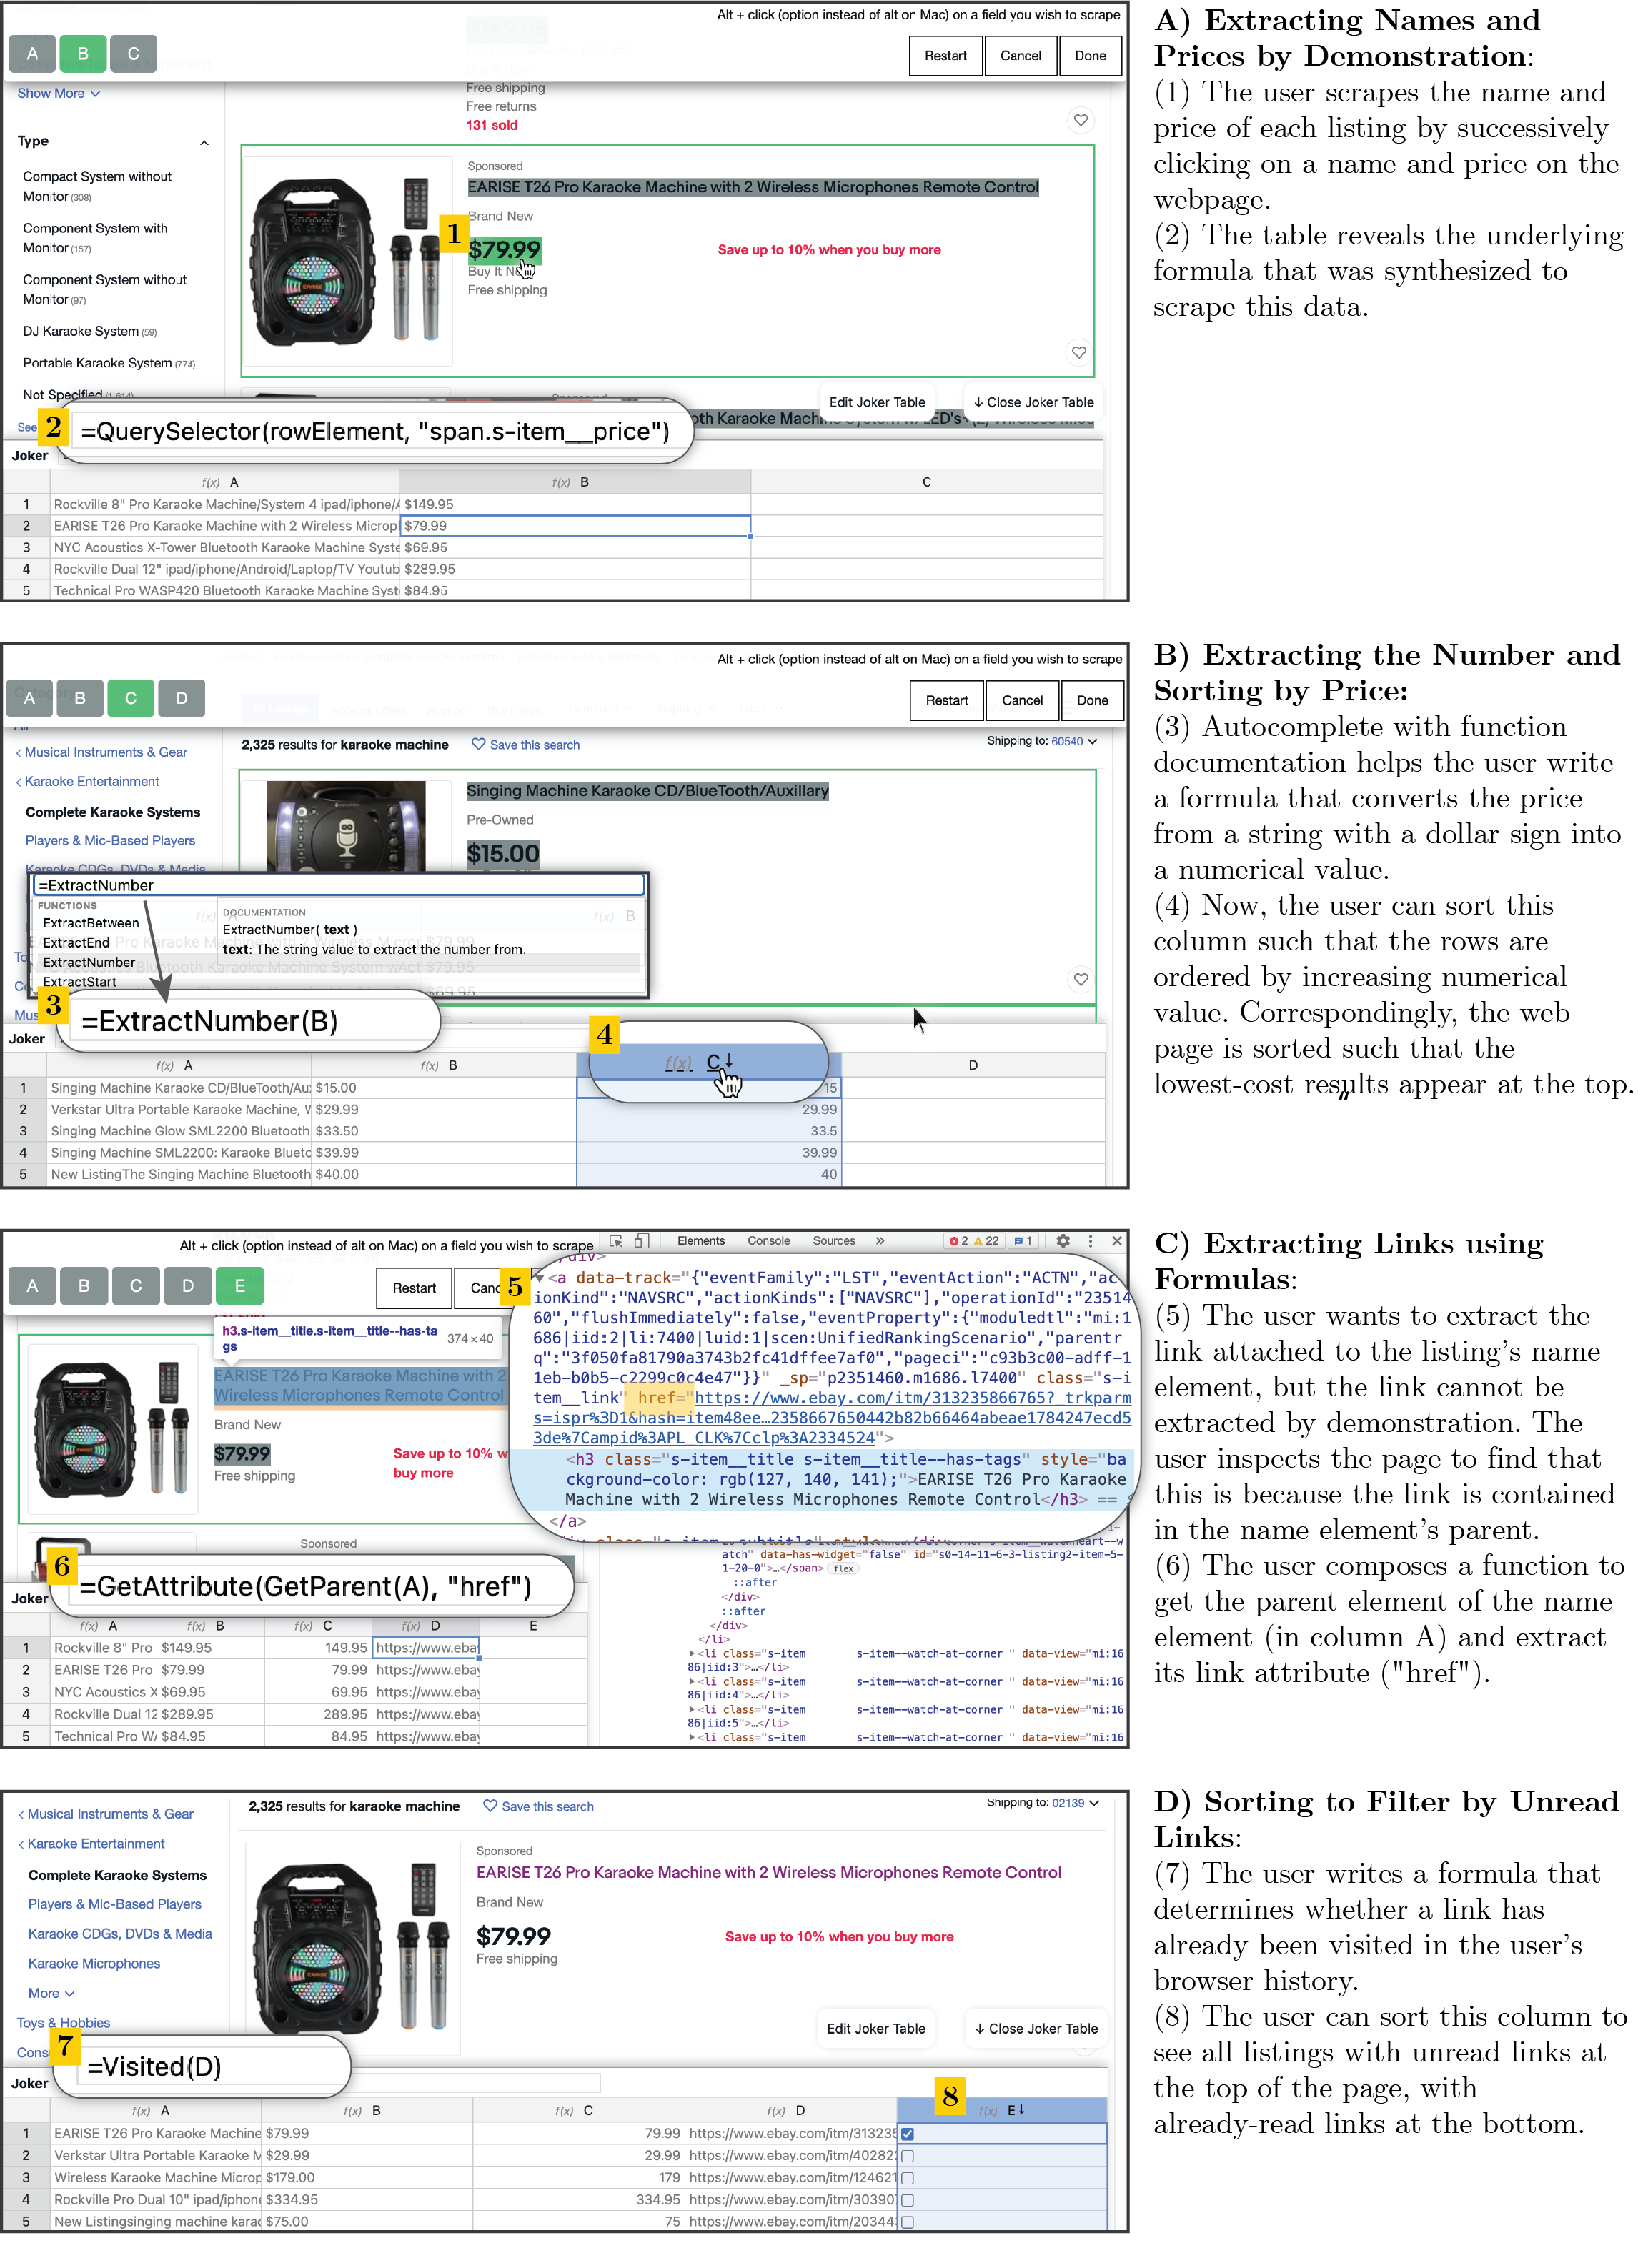
\includegraphics[width=\textwidth]{media/ebay.png}
  \caption{\label{fig:ebay}Scraping and customizing eBay by unified demonstration and formulas.}
\end{figure*}

\textbf{A PBD interface for creating extraction formulas}: Directly
writing extraction formulas can be challenging for end-users, so Joker
provides a PBD interface that synthesizes formulas from user
demonstrations. A key aspect of our design is that the program
synthesized from the demonstration is made visible as a spreadsheet
formula that can be subsequently edited by the user, and is more easily
understood than imperative code due to its declarative form.

Section~\ref{sec:examples} describes a concrete scenario, showing how
Joker enables a user to complete a useful customization task. In
Section~\ref{sec:implementation}, we briefly describe the implementation
of our formula language and user interface, as well as the algorithms
used by our PBD interface.

We have performed two evaluations of our approach, presented in
Section~\ref{sec:evaluation}. First, we describe a suite of case studies
in which we used Joker to extract and augment a variety of websites in
order to characterize its capabilities and limitations. Second, we
describe a formative user study with five participants, which showed
that users were generally able to use Joker to perform useful extraction
and augmentation tasks, but which also uncovered limitations,
particularly for less experienced users trying to extract data from more
complex websites.

Joker relates to existing work not only in end-user web customization,
but also in end-user web scraping and program synthesis, which we
discuss in Section~\ref{sec:related-work}. Finally, we discuss
opportunities for future work in Section~\ref{sec:conclusion}.

\hypertarget{sec:examples}{%
\section{Example Usage Scenario}\label{sec:examples}}

This section describes an example scenario, illustrated in
Figure~\ref{fig:ebay}, and demonstrated in the video accompanying this
paper. Jen is searching for a karaoke machine on eBay, a shopping
website. She wants to use Joker to sort products by price within a page
of search results, a feature not supported by eBay. Because Joker
supports interleaving extraction and augmentation tasks on the fly, Jen
is also able to extract the URLs of products to determine whether they
have been visited and use that to further sort the products. While we
have described only a single illustrative scenario in this example,
Joker is flexible enough to support a wide range of other useful
customizations and workflows on various websites, described in more
detail in Section~\ref{sec:evaluation}.

\hypertarget{sec:implementation}{%
\section{System Implementation}\label{sec:implementation}}

\begin{figure*}
  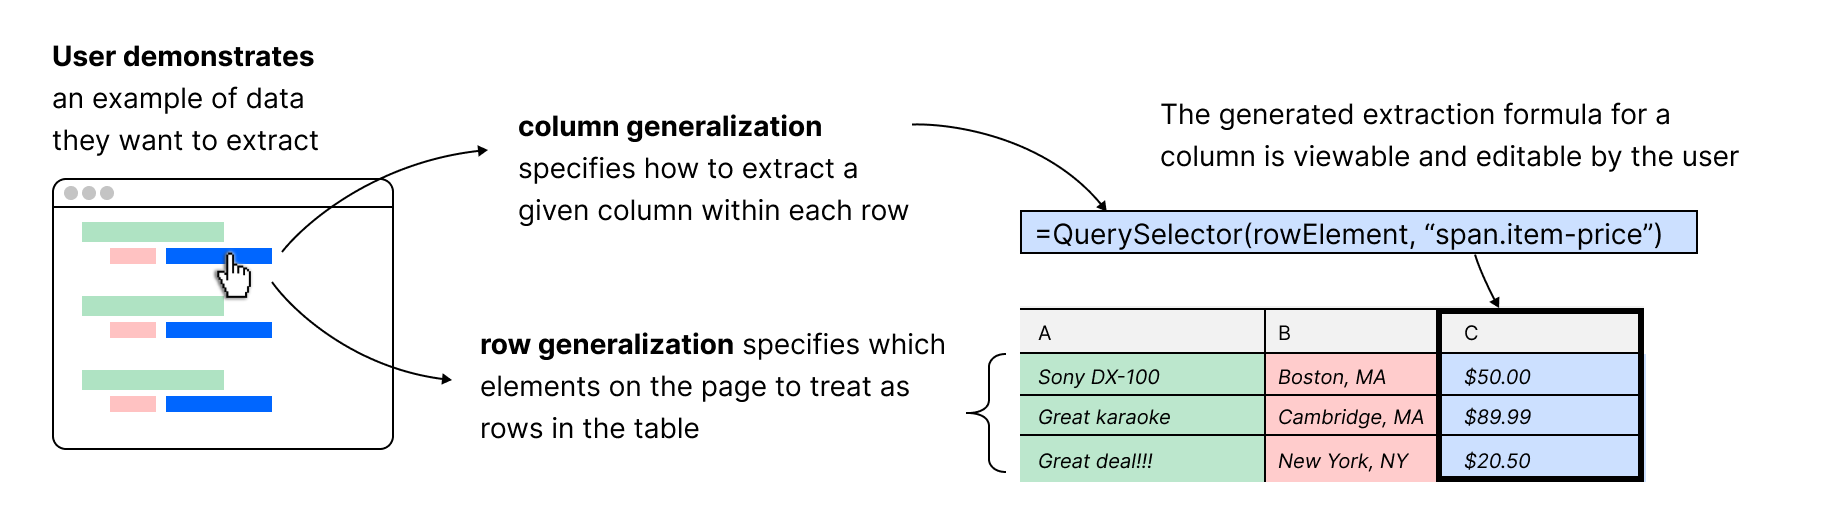
\includegraphics[width=\textwidth]{media/overview.png}
  \caption{\label{fig:overview}An overview of Joker's interaction model and wrapper induction process.}
\end{figure*}

In this section, we briefly describe Joker's formula language and the
\emph{wrapper induction} \citep{kushmerick2000} algorithm that Joker's
PBD interface uses to synthesize the row element and column selectors
presented in formulas. Figure~\ref{fig:overview} illustrates the entire
process.

\hypertarget{extraction-formulas}{%
\subsection{Extraction Formulas}\label{extraction-formulas}}

The Wildcard customization tool includes a formula language for
augmentation, including operators for basic arithmetic and string
manipulation, as well as more advanced operators that fetch data from
web APIs. As in other tabular interfaces like SIEUFERD \citep{bakke2016}
and Airtable \citep{2021f}, formulas apply to a whole column at a time
rather than a single cell, and can reference other columns by name.
Joker extends this base language with new constructs which enable it to
apply to \emph{data extraction} instead of just augmentation. More
information can be found in Appendix A.

By providing a single formula language to express extractions and
augmentations, Joker enables a \emph{unified interaction model} that
supports interleaving the two. Furthermore, the formula language enables
users to specify logic using pure, stateless functions that reactively
update in response to upstream changes. This \emph{functional reactive
paradigm} is easier to reason about than traditional imperative
programming, as demonstrated by the use of formulas by millions of end
users in spreadsheet programs and end-user programming environments
\citep{2021g, 2021h, 2021f, 2021a, 2021c, chang2014}.

\hypertarget{wrapper-induction}{%
\subsection{Wrapper Induction}\label{wrapper-induction}}

When users demonstrate a specific column value to extract, Joker must
synthesize a program that reflects the user's general intent. This is an
instance of the \emph{wrapper induction} problem of synthesizing a web
data extraction query from examples. Prior work on this topic
\citep{kushmerick2000, furche2016} prioritizes accuracy and robustness
to future changes, which makes sense for a fully automated system, but
can lead to very complex queries. In our work, we chose to prioritize
the readability of queries by less sophisticated users, so that users
can more easily author queries and repair them when they break. We
implemented a set of heuristics inspired by Vegemite \citep{lin2009} for
wrapper induction, outlined in Appendix B.

\hypertarget{sec:evaluation}{%
\section{Evaluation}\label{sec:evaluation}}

We evaluate our interaction model and tool in terms of two research
questions:

\emph{RQ1: What kinds of websites can this model operate effectively
on?} We evaluate this with a suite of case studies that demonstrate its
capabilities and limitations.

\emph{RQ2: How are users of different backgrounds able to use the
system?} We evaluate this with a small formative user study.

\hypertarget{case-studies}{%
\subsection{Case Studies}\label{case-studies}}

Our first evaluation describes the results of our use of Joker to
extract data and perform customizations on popular websites.

\hypertarget{successful-applications}{%
\subsubsection{Successful Applications}\label{successful-applications}}

We have used Joker to achieve a variety of customizations across many
websites.

\emph{Sorting search results by price on Amazon.} We have found Joker to
be useful for sorting the contents of various websites. One example of a
useful sort achieved by Joker is sorting search results by price within
the Featured page on Amazon. (Using Amazon's sort by price feature often
returns irrelevant results.) In Amazon's source code, the price is split
into three HTML elements: the dollar sign, the dollar amount, and the
cents amount. A user can extract by demonstration only the cents element
into column \texttt{A}. Subsequently, because the parent element of the
cents element contains all three of the price elements, the user can
extract the full price using the formula \texttt{GetParent(A)}. Next,
the user can write the formula \texttt{ExtractNumber(B)} to convert the
string into a numeric value. Finally, the user can sort this column by
low-to-high prices. In a similar manner, we have used Joker to extract
and sort prices and ratings on the product listing pages of Target and
eBay.

\emph{Filtering titles of publications on Google Scholar.} We have also
found Joker can be useful for filtering a website's listings based on
the text content of an element in the listing. For example, we have used
Joker to filter the titles of a researcher's publications on their
Google Scholar profile which is not natively supported. First, a user
can extract the titles into a column (\texttt{A}) by demonstration.
Then, the user can write the formula \texttt{Includes(A,\ "compiler")}
that returns whether or not the title contains the keyword ``compiler.''
Finally, the user can sort by this column to get all of the publications
that fit their constraint at the top of the page. We have also used
Joker to filter other text-based directory web pages such as Google
search results and the MIT course catalog, in similar ways.

\emph{Retrieving information about links on Reddit.} Additionally, we
have used Joker to augment web pages with external information. For
example, Joker can augment Reddit's user interface, which has a list of
headlines with links to articles, with the links' read times and whether
the link has already been read. To achieve this customization, a user
first extracts the headline elements into column (\texttt{A}) by
demonstration. The user can then extract the link into the next column
(\texttt{B}) with the formula \texttt{GetAttribute(A,\ "href")}. Then,
the user can write the formula \texttt{ReadTimeInSeconds(B)} that calls
an API that returns the links' read times. Similarly, the user can write
the formula \texttt{Visited(B)}, which uses another API that returns
whether that link has been visited in the user's browser history. The
user can also extract elements such as the number of comments and the
time of posting and sort by these values. We have performed similar
customizations on websites such as ABC News and CNN.

\hypertarget{limitations}{%
\subsubsection{Limitations}\label{limitations}}

Joker is most effective on websites whose data is presented as a
collection of similarly-structured HTML elements. Certain websites,
however, have designs that make it difficult for Joker to extract data:

\begin{itemize}
\tightlist
\item
  \emph{Heterogeneous row elements.} Some websites break their content
  into rows, but the rows do not have a consistent layout, and contain
  different types of child elements. For example, the page design of
  HackerNews alternates between rows containing a title and rows
  containing supplementary data (e.g.~number of likes and the time of
  posting). Because Joker only chooses a single row selector, when
  extracting by demonstration, Joker will only select one of the types
  of rows, and elements in the other types of rows will not be
  extracted.
\item
  \emph{Infinite scroll.} Some websites have an ``infinite scroll''
  feature that adds new entries to the page when a user scrolls to the
  bottom. Joker's table will only contain elements that were rendered
  when the table was first created. Additionally, for websites that
  render a very large number of DOM elements, the speed of the live
  feedback provided by Joker's PBD interface might significantly
  decrease. This is because the wrapper induction process used by the
  PBD interface queries the DOM which takes longer as the size of the
  DOM increases.
\end{itemize}

\hypertarget{user-study}{%
\subsection{User Study}\label{user-study}}

Our second evaluation reports a small, formative user study we conducted
to understand how users would interact with Joker.

\hypertarget{participants}{%
\subsubsection{Participants}\label{participants}}

We recruited 5 participants with varying backgrounds. 3 participants
were familiar with spreadsheet formulas. 3 participants had extensive
web development experience, 1 had a small amount of prior web
development experience, and 1 had no web development experience. 3
participants had previously extracted data from websites.

\hypertarget{protocol}{%
\subsubsection{Protocol}\label{protocol}}

The participants completed 7 web customization tasks across 2 websites.
All participants attempted all the tasks.

First, we asked participants to customize a website with a relatively
simple HTML structure: the MIT EECS course catalog website. All data
\emph{extraction} on this site can be performed with demonstrations
alone in Joker, although augmentation still requires writing formulas.
The specific tasks were the following: 1a) Extract course titles, 1b)
Extract course prerequisites, 1c) Add a column that indicates whether a
course has a prerequisite \& 1d) Add a column that indicates whether a
course has no prerequisites and is offered in the fall term.

Next, we asked participants to customize a website with a more complex
HTML structure: the search results page for the eBay shopping website.
Due to the website's complexity, demonstrations alone are not sufficient
to extract data; users must also directly edit extraction formulas. The
specific tasks were the following: 2a) Extract title from listings of
Apple iPhones for sale, 2b) Extract the listing price for the phone, \&
2c) Create a column that indicates whether a listing for a phone is
sponsored.

Each session was 60 minutes long and conducted over a recorded video
conference. We started each session with a description of Joker and
provided a brief tutorial of its main features on a sample website not
used in the tasks. There was no time limit for completing the tasks.
Users were encouraged to speak aloud as they worked.

Because some of the tasks build on results of previous tasks, we wanted
to ensure all participants made enough progress to gather useful
feedback. Therefore, whenever a participant got stuck for several
minutes, we recorded why they were stuck and then offered hints on how
to proceed (such as suggestions to read formula documentation or open
the browser dev tools). While all participants were able to complete all
tasks with hints, this obviously does not mean they could have completed
the task unassisted. Our goal was not to simply measure whether users
completed the task, but rather to gain qualitative insight into the
barriers they faced.

\hypertarget{results}{%
\subsubsection{Results}\label{results}}

We have categorized our results into the following four groups:

\emph{Unified interaction model.} Most participants took advantage of
the unified interaction model to interleave extraction and augmentation
tasks, rather than performing all extraction up front. For example, on
task 1, most participants extracted the prerequisites by demonstration,
added one or more columns to the table to perform some string operations
on the prerequisites, and then continued on to extract more information
from the web page by demonstration. Furthermore, we hypothesize that in
a less controlled setting, users would be even more likely to interleave
extraction and augmentation, since the task may be less well defined at
the beginning.

One usability issue with the unified model was that participants
sometimes got confused about how their demonstrations would affect the
contents of the table. For example, multiple participants intended to
add a new column by demonstrating an extraction, but instead
accidentally overwrote the contents of an existing column. This poses a
design challenge because the user's demonstrations occur in the website,
so they cannot directly interact with the table while demonstrating;
this suggests that the interface needs to do a better job indicating
where the results of a demonstration will be inserted.

\emph{Extracting simple data.} On the relatively simple MIT course
catalog website, all participants were able to extract the relevant data
from the page within seconds, simply performing demonstrations with a
few clicks. This suggests that when Joker's generalization algorithm
works well, it can be an effective tool for data extraction, even for
users with limited programming experience. P1 said: \emph{``you could
hover and {[}the data{]} was already selected\ldots that was very
nice''}. P3, upon seeing the tutorial for extraction by demonstration,
said \emph{``that's like black magic.''}

\emph{Extracting complex data.} On the more complex eBay website where
demonstration alone was not sufficient, results were more varied. P1,
who had no prior web development experience, struggled to complete the
task, saying that \emph{``looking at HTML is a bit much''}; this
suggests that more work could be done to make the experience usable for
novices. However, users with more web development experience were able
to use the tool to perform complex extractions, such as directly writing
CSS selectors into the formula bar. P2 and P3 both reported that Joker's
live feedback loop was easier to use and faster than other approaches to
web extraction; P3 noted that \emph{``{[}with any other approach{]}, it
would have been slower to specify and slower to validate that I
specified it correctly.''}

It was challenging for some participants to switch between using the
browser's developer tools and the Joker interface when doing complex
extraction tasks. While we chose not to build HTML inspection into the
Joker UI because the browser already provides a very rich set of tools,
users sometimes were not able to tell how elements in the Joker table
corresponded to elements in the browser's element inspector.

\emph{Writing formulas.} In general, participants were able to learn the
formula language by using an autocomplete dropdown with inline
documentation, which we developed as part of the Joker extension. In
some cases, participants were able to immediately construct correct
formulas on the first try; in other cases it took several attempts and
some hints from the moderator to try a relevant function. While better
documentation and error messages could help improve the learnability of
the formula language, we also did not find it surprising that
participants required some time to learn a completely unfamiliar formula
language.

\hypertarget{sec:related-work}{%
\section{Related Work}\label{sec:related-work}}

\hypertarget{end-user-web-customization}{%
\subsection{End-user Web
Customization}\label{end-user-web-customization}}

Joker builds on web customization ideas implemented by previous tools.
Our contribution is a new interaction model that allows for interleaving
extraction and augmentation, enabled by a unified formula language and a
PBD interface.

Joker is an extension of the Wildcard customization system
\citep{litt2020}, and preserves its foundational idea of synchronizing a
table with a website. Wildcard only allows for extraction logic to be
written by programmers in Javascript; our work has substantially
extended the Wildcard formula language and added an entire new system
for dynamically creating data extraction logic within the user
interface. We also improved the formula editing interface by adding an
autocomplete dropdown and documentation popup, which proved important in
our testing for allowing end-users to reliably edit and create formulas.

Vegemite \citep{lin2009} is a tool for end-user programming of web
mashups. Like Joker, it allows users to perform demonstrations to
extract data, but Vegemite only displays a table after all the
demonstrations have been provided, which rules out interleaving
extraction and augmentation. Vegemite does allow users to directly view
and edit some of the logic generalized from demonstrations, but it only
allows for editing augmentation logic, not extraction logic. The wrapper
induction algorithm used in Joker is also very similar to Vegemite's
algorithm.

Sifter \citep{huynh2006} is a tool that augments websites with advanced
sorting and filtering functionality. It attempts to automatically detect
items and fields on the website with a variety of heuristics. If these
fail, it gives the user the option of demonstrating to correct some
parts of the result. In contrast, Joker makes fewer assumptions about
the structure of websites, by giving control to the user from the
beginning of the process and displaying an editable synthesized program.

\hypertarget{end-user-web-scraping-and-program-synthesis}{%
\subsection{End-user Web Scraping and Program
Synthesis}\label{end-user-web-scraping-and-program-synthesis}}

Joker builds on insights from other tools that synthesize web scraping
(i.e.~data extraction) code from user demonstrations, and give users
ways to inspect and modify the generated code.

Rousillon \citep{chasins2018} is a tool that enables end-users to
extract hierarchical web data across multiple linked web pages. It
presents the web extraction program generated from demonstrations in an
editable, high-level, block-based language called Helena \citep{2021c}.
While both Rousillon and Joker create an editable program, they have
different focuses. Because Rousillon allows users to extract data across
multiple pages (e.g., extracting details from each linked page in a
list), it uses an imperative language, with nested loops as a key
construct. In contrast, Joker can only extract within a single page, and
therefore can use a simpler declarative formula language. Also,
Rousillon only allows editing high-level control flow and treats some
details of the extraction logic as opaque; Joker offers finer-grained
control over details like CSS selectors.

Mayer et al propose a user interaction model called \emph{Program
Navigation} \citep{mayer2015} which aims to give users another mechanism
beside examples for guiding the generalization process of PBE tools like
FlashExtract \citep{le2014} and FlashFill \citep{harris}. This is
important because demonstrations are an ambiguous specification for
program synthesis \citep{peleg2018}: the set of synthesized programs for
a demonstration can be very large. Joker shares the general idea of
displaying synthesized programs, but only presents the top-ranked
program. More broadly, Joker's use of PBD to generate editable code
embodies Ravi Chugh's notion of \emph{prodirect manipulation}
\citep{chugh2016a}, implemented in Sketch-N-Sketch \citep{chugh2016},
which aims to bridge the divide between programmatic and direct
manipulation.

\hypertarget{sec:conclusion}{%
\section{Conclusion And Future Work}\label{sec:conclusion}}

In this paper, we presented a unified interaction model for web
customization. Our key idea is a spreadsheet formula language that
encompasses both extraction and augmentation tasks, along with a
programming-by-demonstration (PBD) interface that makes it easy for
end-users to program to create formulas. The main area of future work
involves making the formula language more accessible to end-users not
familiar with CSS selectors. Our ultimate goal is to enable anyone that
uses the web to customize websites in the course of their daily use in
an intuitive and flexible way.

\newpage

% \printbibliography

%%
%% The next two lines define the bibliography style to be used, and
%% the bibliography file.
\bibliographystyle{ACM-Reference-Format}
\bibliography{references-bibtex.bib}

\clearpage
\hypertarget{appendix}{%
\section*{Appendix}\label{appendix}}

\hypertarget{appendix-a}{%
\subsection*{A: Extraction Formulas}\label{appendix-a}}

Joker adds DOM elements as a data type to Wildcard's formula language, alongside strings,
numbers, and booleans. Because the language runs in a JavaScript
interpreter, we simply use native JavaScript values to represent DOM
elements in the language. DOM elements are displayed visually by showing
their inner text contents. They can also be implicitly typecast to
strings for use in other formulas; for example, a string manipulation
formula like \texttt{Substring} can be called on a DOM element value,
and will operate on its text contents.

We also added several functions to the formula language for traversing
the DOM and performing extractions, summarized below with their types:

\begin{itemize}
\tightlist
\item
  \texttt{QuerySelector(el:\ Element,\ sel:\ string):\ Element}.
  Executes the CSS selector \texttt{sel} inside of element \texttt{el},
  and returns the first matching element.
\item
  \texttt{GetAttribute(el:\ Element,\ attribute:\ string):\ string}.
  Returns the value for an attribute on an element.
\item
  \texttt{GetParent(el:\ Element):\ Element}. Returns the parent of a
  given element.
\end{itemize}

To extract data from a row, formulas need a way to reference the current
row, so we added a construct to support this use case. Every row in the
table maps to one DOM element in the page; we allow formulas to access
this DOM element via a special keyword, \texttt{rowElement}. In some
sense, \texttt{rowElement} can be seen as a hidden extra column of data
in the table containing DOM elements.

While many more functions could be added to expose more of the
underlying DOM API, we found that in practice these three functions
provided ample power through composition. For example, in
Section~\ref{sec:examples} we showed how \texttt{GetParent} and
\texttt{GetAttribute} can be composed to traverse the DOM and extract
the URL associated with a product listing.

\hypertarget{appendix-b}{%
\subsection*{B: Wrapper Induction Algorithm}\label{appendix-b}}

Our wrapper induction algorithm implements a set of heuristics inspired by Vegemite
as described below:

\hypertarget{determining-row-elements}{%
\subsubsection*{Determining Row
Elements}\label{determining-row-elements}}

The user starts by demonstrating an element \(v\), representing a value
that should be in the table. From that demonstration, we must find a set
of \emph{row elements} that represent the rows of the table. We could
naively assume that \(parent(v)\) is the row containing \(v\), but often
\(v\) is deeply nested inside its containing row; we must determine
which ancestor of \(v\) is likely to be the row.

Intuitively, we solve this problem by assuming that all rows share some
similar internal structure. In particular, we expect most rows to
contain a value for the demonstrated column. (If there were no missing
data, we'd expect \emph{all} rows to contain data for this column.)

Formally: assume a function \(select(el, s)\) which runs a CSS selector
that returns the set of elements matching \(s\) within \(el\). We
generate a set of plausible candidates \(P\), consisting of pairs of a
row element and a CSS selector:

\(P = \{ (r, s) \mid r \in ancestors(v) \land select(r, s) = \{v\} \}\)

For each candidate \((r, s) \in P\), we compute a weight function \(w\),
which is based on the number of siblings of \(r\) that have ``similar
structure'', defined by checking whether running \(s\) within the
sibling also returns a unique element.

\(w(r, s) = |\{ r' \mid r' \in siblings(r) \land |select(r', s) | = 1 \}|\)

We then choose the candidate with the highest weight. In case of ties,
the candidate closer to \(v\) in the tree (i.e., lower in the tree)
wins. Given a winning candidate \((r, s)\), the full set of row elements
is \(\{r\} \cup siblings(r)\).

\hypertarget{synthesizing-css-selectors-for-column-values}{%
\subsubsection*{Synthesizing CSS Selectors For Column
Values}\label{synthesizing-css-selectors-for-column-values}}

Once we have determined the row elements, next we must choose a CSS
selector that will be used to identify the demonstrated value within its
row.

Given a demonstrated value \(v\) within a row element \(r\), we generate
two kinds of plausible selectors:

\begin{itemize}
\tightlist
\item
  selectors using CSS classes, which are manual annotations on DOM
  elements added by the website's programmers, typically for styling
  purposes (e.g.~"item\_\_price")
\item
  selectors using positional indexes within the tree, using the
  \texttt{nth-child} CSS selector (e.g.~\texttt{nth-child(2)},
  representing the second child of an element)
\end{itemize}

The minimum criteria for a plausible selector \(s\) is that it uniquely
identifies the value within the row: \(select(r, s) = \{v\}\). But there
may be many plausible selectors, so we must pick a best one.

We first prioritize selectors using classes, because they tend to be
more robust to changes on the website. A single selector can combine
multiple classes, but we prefer using fewer classes when possible. If no
plausible class-based selector can be generated (for example, if the
relevant elements don't have any classes to query), we fall back to
using a positional index selector. This kind of selector can always be
generated regardless of the contents of the page, but tends to be less
accurate and robust.

\end{document}
\endinput
%%
%% End of file `sample-sigconf.tex'.
